\chapter{Análisis Experimental}
En esta sección se presenta la descripción de los escenarios , la plataforma de ejecución y el análisis experimental.

Este se divide en dos etapas, primero se realiza la configuración parametrica para encontrar la mejor ejecución del algoritmo. Luego se realizan las pruebas donde se comparan los resultados entre los distintos escenarios.






\section{Desarrollo y Plataforma de ejecución }
Los algoritmos fueron desarrollados usando la librería Malva que fue extendida en el código base para soportar la creación de nuevos hilos de ejecución para lograr el funcionamiento en paralelo.


Los escenarios fueron ejecutados en el cluster fing.

Cluster: Es un conjunto de computadoras independientes conectadas para que trabajen integradas como un solo sistema. De esta forma se consigue un alto rendimiento en la ejecución de tareas. 

Cluster Fing: Es una infraestructura de alto desempeño, que brinda soporte en la resolución de problemas complejos que demandan un gran poder de computo.

Descripcion del hardware: 
\begin{itemize}
	\item 9 servidores de cómputo
	\subitem Quad core Xeon E5430, 2x6 MB caché, 2.66GHz, 1.333 MHz FSB.
	\subitem 8 GB de memoria por nodo.
	\subitem Adaptador de red dual (2 puertos Gigabit Ethernet).
	\subitem  Arquitectura de 64 bits.
	\subitem Servidor de archivos: 2 discos de 1 TB, capacidad ampliable a 10 TB.
	\subitem Nodos de cómputo: discos de 80 GB.
	\item Switch de comunicaciones
	\subitem Dell Power Connect, 24 puertos Gigabit Ethernet.
	\item Switch KVM (16 puertos) y consola.
	\item UPS APC Smart RT 8000VA.
\end{itemize}

\section{Ajuste de parámetros de algoritmos}
Se busca la mejor configuración inicial de los parámetros realizando pruebas experimentales con diferentes combinaciones.  

\begin{itemize}
	\item Tiempo de simulación	
	\item Criterio de parada
	\item Tamaño de la población
	\item Probabilidad de mutación
	\item Probabilidad de cruzamiento
\end{itemize}

Para la realización de las pruebas se generan tres instancias con densidades de tráfico diferentes para realizar las pruebas de configuración. De esta forma el algoritmo queda generico y no sesgado a un caso en particular. Se representa la cantidad de ómnibus y otros vehículos que circulan por la zona de Garzon en un tiempo de una hora. El caso de tráfico medio representa una aproximación de los datos obtenidos in-situ.

\begin{itemize}
	\item Tráfico Bajo: 30 ómnibus y 500 vehículos	
	\item Tráfico Medio: 60 ómnibus y 1000 vehículos
	\item Tráfico Alto: 120 ómnibus y 2000 vehículos
\end{itemize}

En general se realizan 21 pruebas individuales en cada prueba para lograr mejor confiabilidad estadística, 7 para cada una de las densidades de tráfico.

En este proceso primero se define el tiempo de simulación y el criterio de parada, luego de establecidos se realizan las pruebas para todas las combinaciones de tasa de cruzamiento y mutación buscando los mejores valores para optimizar el algoritmo.


Al estas utilizando un cluster tenemos a nuestra disposición tanto la métrica del tiempo real que llevo la ejecución, así como también el tiempo secuencial es decir la suma del tiempo de procesamiento de todos los procesadores involucrados en la evaluación del algoritmo. 
A saber en las comparaciones del tiempo de ejecución se refiere al tiempo secuencial que es más confiable al no tener el sesgo dado por la cantidad de procesadores utilizados en la evaluación.
En general para las diversas pruebas se utilizaron entre 16 y 64 procesadores.




\subsection{Tiempo de simulación}

Para tener un mejor control sobre los tiempos totales de ejecución, se busca encontrar un número fijo para el tiempo de la simulación de cada escenario que se ejecutara para cada solución.

Teniendo en cuenta que cada simulación de los escenarios representan el tráfico vehicular durante una hora real y que se valido que en cada escenario más de los 80 \% de los vehículos hayan dejado la simulación, es decir llegado a sus destinos.

Se establece un tiempo de simulación de 4000 steps (medida interna de tiempo del simulador SUMO equivalente a 66 minutos reales) que cumple con los criterios establecidos. 

\subsection{Criterio de Parada}
Se elige como criterio de parada el número de generación, esto permite estandarizar las pruebas para una mejor comparación.

Para determinar el número de generación donde parar el algoritmo se busca un compromiso entre un buen resultado y un tiempo de ejecución apropiado que no sea excesivo.

Para esto se decide que por un lado la ejecución del algoritmo deberá estar comprendida entre 1h y 24h y además comprobar experimentalmente que el valor de fitness no tiene una gran variación en las ultimas 100 generaciones.

Luego de la realización de las pruebas se elige el número de 500 generaciones como criterio de parada, como se ve en la siguiente gráfica representativa de las pruebas realizadas se aprecia como el valor de fitness no presenta grandes variaciones luego de la generación 400.


\begin{figure}[h]
\centering
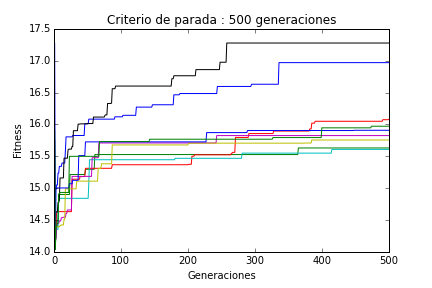
\includegraphics[width=0.7\linewidth]{Figures/criterio_parada}
\caption{Resumen representativo de ejecuciones del algoritmo para establecer el criterio de parada.}
\label{fig:criterio_parada}
\end{figure}



\subsection{Tamaño de la población}

Para la elección de la población se tendrán en cuenta 3 elementos. El valor de fitness encontrado, el tiempo de ejecución total y la plataforma de ejecución.

Dado que estamos ejecutando en el cluster y la máxima cantidad de procesadores que se pueden utilizar son 64 en un mismo nodo y teniendo en cuenta que la mejor distribución del trabajo es un elemento de población por procesador, se tiene que la máxima cantidad de población que estudiaremos sera 64.

Luego se eligen los valores 32 y 48 para completar el análisis teniendo en cuenta que no son lo suficientemente bajos como 8 u 16 y son valores con los que se obtiene una distribución más adecuada.

La siguiente tabla muestra los resultados obtenidos, como se aprecia no existen grandes diferencias en la elección de un número poblacional sobre otro. Por tanto se elige como número de población 32 teniendo en cuenta el tiempo de ejecución secuencial del algoritmo que como se aprecia es el menor. Se elige esta métrica por que aunque al ejecutar en paralelo el tiempo real que se puede obtener utilizando la máxima cantidad de procesadores para cada población son similares también se tiene en cuenta la disponibilidad y utilización de recursos que insume en el cluster fing. Por ejemplo obtener 64 procesadores para utilizar por un proceso en el cluster es algo que puede demorar varios dias por la cantidad de otros procesos que también están funcionando en la plataforma y como se ve la ganancia que tenemos es mínima.

\begin{table}
	\renewcommand{\arraystretch}{1.2}
	\caption{Comparación de fitness para distintas poblaciones}
	\label{table:parametro_poblacion}
	\centering
	\begin{tabular}{ccrrcr}
		\hline
		\multirow{2}{*}{\textbf{población}} & & 
		\multicolumn{2}{c}{\textbf{Fitness}} \\
		\cline{3-4}
		& & \multicolumn{1}{c}{mejor} 
		& \multicolumn{1}{c}{promedio} 
		& \multicolumn{1}{c}{tiempo de ejecución(m)} \\
		\hline
		32 & & \textbf{17.28} & 16.37$\pm$0.5 & 4853\\
		48 & & \textbf{16.19} & 15.84$\pm$0.3 & 6772\\
		64 & & \textbf{17.27} & 16.46$\pm$0.6 & 10184\\
		\hline
	\end{tabular}
\end{table}




\subsection{Probabilidad de mutación y cruzamiento}

Los valores elegidos fueron:

\begin{itemize}
	\item Probabilidad de cruzamiento (pc):  0.5, 0.8, 1
	\item Probabilidad de  mutación (pm):  0.01, 0.05, 0.1
\end{itemize}

Se prueban todas las combinaciones  de cruzamiento y mutación.

En las siguientes figuras se muestran los valores de fitness obtenidos en cada caso.


INSERTAR GRAFICA de los 3 casosd de tráfico.

En estos resultados podemos observar la influencia de estos parametros a la hora de obtener una buena solución.

La combinacion 0.4 de mutacion y 05 de cruzamiento es la que obtiene mejor rendimiento en los tres casos por lo que la elegimos como parametros del algoritmo.

La mejor  configuración obtenida fue:
Población:120, mutación:0.01 , cruzamiento: 1

Las gráficas muestras el promedio de las 20 ejecuciones para resolver el escenario inicial.





\section{Descripción de escenarios}
En todos los escenarios se utiliza los datos obtenidos del tráfico vehicular, configuración de semáforos y frecuencia de los ómnibus obtenidos. 

\subsection{Caso base}
Esto representa la situación actual en términos de tráfico, red vial y sincronización de semáforos del corredor Garzón. 

Se valida su correctitud comparando los tiempos obtenidos en la simulación con tiempos obtenidos in-situ de los recorridos de ida y vuelta para los vehículos. Y utilizando las frecuencias de acceso publico en el caso de los ómnibus.

\subsection{Escenario Evolutivo }
En este caso se ejecuta el algoritmo evolutivo sobre el caso base para obtener una nueva sincronización de semáforos optimizada que repercutirá en la calidad del tráfico.

\subsection{Escenario Alternativo}
Luego de analizar aquellos puntos que se entienden podrían atentar contra el buen funcionamiento del Corredor, se agregan algunas modificaciones al escenario base para intentar mejorarlo. 

-Limitar cruces a la izquierda

-Eliminar paradas

-Agregar calles paralelas a Garzon

-


\section{Resultados}
Presentaremos los resultados obtenidos  utilizando los parámetros óptimos  para el escenario inicial, el escenario modificado, y la prueba en el cluster.

\subsection{Resultado simulación caso base}
El caso base se construye a partir del modelo de tráfico con los datos tomados in-situ por lo que muestra valores aproximados de la realidad actual.

En este caso tenemos las siguentes metricas

Tiempo de viaje promedio de ida en un vehiculo
Tiempo de viaje promedio de ida en omnibus por el corredor:
Velocidad promedio de los vehiculos:
Velocidad promedio de los omnibus:

Estas metricas seran las que utilizaremos para comparar con los resultados luego de aplicar el algoritmo.

\subsection{Resultado Escenario Evolutivo}
\subsection{Resultado Escenario Alternativo}

\subsection{Comparación caso base vs Algoritmo Secuencial}
Análisis comparativo : test paramétrico
H1)  los  resultados  de  mejor  fitness  tienen  una distribución normal.
H2)Existe  una  diferencia  significativa  entre  los  de conjuntos  de  muestras  obtenidos  por  el  algoritmo  y  la realidad.

El  test  de  normalidad  de  Shapiro-Wilks  resultó  ser verdadero  en  ambos  casos  con  un  alto  porcentaje  de
confiabilidad y luego al realizar los test T-student resulto tener menos de 0,0001 lo que se considera una diferencia que
estadísticamente  es  significativa.  Esto confirma algo que resulta evidente ya que al comparar
el promedio de los mejores fitness con la realidad encontramos
una diferencia de un 31,8% y un 15% respectivamente y estos
casos  son  bastante  acotados  ya  que  hay  mucha  cantidad  de
vehículos con grandes/medias distancias.

Con  los  resultados  obtenidos  en  las  ejecuciones  para  los
escenarios  1  y  2  se  obtuvo  un  mejor  fitness  de  661  y  515
respectivamente, comparado con el tiempo de la configuración
real que demora 1019 y 690, las soluciones son muy buenas.



\subsection{Comparación Secuencial vs  Paralelo}

El speedup se define como T1/Tp
T1 es el tiempo de ejecucion en un procesador
Tp es el tiempo de ejecucion en p procesdores.


Vamos a comprobar la utilidad de tener un algoritmo paralelo comparando el tiempo de ejecucion en diferentes número de procesadores

La escabilidad de un algoritmo define su capacidad para aumentar su rendimiento a medida que se agregan más procesadores.

En este caso comparamos el algoritmo ejecutado en 1, 8, 16, 32 procesadores.

GRAFICA DE ESCABILIDAD

El comando "time" ejecutado sobre nuestro algoritmo nos brinda el tiempo real de ejecución, así como el tiempo total sumado de todos los procesadores. Por tanto podemos calcular el tiempo del algoritmo secuencial.

En el caso de 8 procesadores, al tener una población de 32 se distribuirán 4 individuos por procesador.

Por tanto cuando tenemos 32 es donde se logra la mejor distribución al no existir "overhead" en la creación y terminación de los hilos.


\section{Resumen}

